\documentclass[10pt, oneside]{article} 
\usepackage{amsmath, amsthm, amssymb, calrsfs, wasysym, verbatim, bbm, color, graphics, geometry}
\usepackage{polski}
\usepackage[utf8]{inputenc}
\usepackage[cache=false]{minted}
\usepackage{algorithm}
\usepackage{algorithmicx}
\usepackage[noend]{algpseudocode}
\usepackage{url}
\usepackage{tikz}
\usepackage{pgfplots}
\usepackage{booktabs}
\usepackage[T1]{fontenc}

\setminted{linenos=true}

\usetikzlibrary{matrix,arrows,automata}

\geometry{tmargin=.75in, bmargin=.75in, lmargin=.75in, rmargin = .75in}  

\theoremstyle{remark}
\newtheorem*{example}{Przykład}


% Cormen's cost analysis
\newcommand{\TITLE}[1]{\item[#1]}
\renewcommand{\algorithmiccomment}[1]{$/\!/$ \parbox[t]{4.5cm}{\raggedright #1}}
% ugly hack for for/while
\newbox\fixbox
\renewcommand{\algorithmicdo}{\setbox\fixbox\hbox{\ {} }\hskip-\wd\fixbox}
% end of hack
\newcommand{\algcost}[2]{\strut\hfill\makebox[1.5cm][l]{#1}\makebox[4cm][l]{#2}}



\title{Algorytmy i struktury danych -- notatki do kursu}
\author{mgr. inż Dominik Filipiak}
\date{Rok akademicki 2019/2020}

\begin{document}

\maketitle
\tableofcontents

\vspace{.25in}

Dokument ten jest pomocą dla prowadzącego i nie zastępuje w żaden sposób podręcznika akademickiego.
W szczególności nauka z tego dokumentu nie jest gwarantem zdania egzaminu.
Dokument powstał głównie na podstawiem książki Cormena i in. \emph{Wprowadzenie do algorytmów}.
Autor nie odpowiada ze ewentualne błędy w tym dokumencie.

\section{Wprowadzenie}

\subsection{O prowadzącym}
Mgr inż. Dominik Filipiak, Katedra Informatyki Ekonomicznej, p 3.24 CEUE (wejście przez 3.33), III piętro.
Strona WWW: \url{http://dfilipiak.com}, e-mail: \url{dominik.filipiak@dalejstandardowo} (proszę zaczynać tytuły wiadomości od [ASD]).
Konsultacje (tylko po wcześniejszym umówieniu się mailowo, minimum 24h wcześniej - wiadomości wpadają często do spamu...): czwartki 16:00-17:00, piątki 12:00-13:00.

\subsection{Egzamin}
Egzamin z przedmiotu (wykład + ćwiczenia) odbędzie się:
\begin{itemize}
	\item I termin: na ostatnich ćwiczeniach 28 i 30 stycznia (w zależności od grupy na moich zajęciach),
	\item II termin: 12 lutego,
	\item III termin: 27 lutego.
\end{itemize}
Progi punktowe określa prof. Abramowicz.
Zaliczenie
Obowiązują ogólne zasady zaliczenia w KIE. Obecność na ćwiczeniach jest obowiązkowa. Każda nieobecność nieusprawiedliwiona począwszy od trzeciej włącznie to ujemne punkty na egzaminie (-3\%).
Zgodnie z regulaminem studiów, przy ponad połowie nieobecności (usprawiedliwionej bądź nie) jestem zmuszony przedstawić taką osobę dyrektorce studiów do skreślenia z listy studentów. Skany usprawiedliwień proszę przesyłać mailem w terminie zgodnych z zasadami zaliczania w KIE.

\subsection{Literatura}
\begin{itemize}
	\item Cormen Thomas H., Leiserson Charles E., Rivest Ronald L, Clifford Stein. \emph{Wprowadzenie do algorytmów}. Wydawnictwo Naukowe PWN, Warszawa, 2018.
	\item Lutz Mark. \emph{Python. Wprowadzenie}. Wydanie IV, Helion, 2011.
	\item Papadimitriou Christos H. \emph{Złożoność obliczeniowa}. Helion, 2012.
\end{itemize}
Większość użytych tu przykładów będzie pochodziła z książki Cormena i reszty.

\section{Proste algorytmy}

Definicja algorytmu, kod a pseudokod.

\subsection{Pierwiastki kwadratowe}
Niech $a,b,c \in \mathbb{R}, a \neq 0$.
Pierwiastki równania kwadratowego o postaci $y=ax+bx+c$ wyliczamy korzystając ze znanego ze szkoły średniej algorytmu.

\begin{algorithm}
    \caption{Pierwiastki rzeczywiste równania kwadratowego}
    \label{euclid}
    \begin{algorithmic}[1] % The number tells where the line numbering should start
        \Function{Quadratic-Roots}{$a, b, c$}
            \State $\Delta \gets b^2 - 4ac$
            \If{$\Delta > 0$} 
            	\State $x_1 \gets \frac{-b - \sqrt{\Delta}}{2a}$
            	\State $x_2 \gets \frac{-b + \sqrt{\Delta}}{2a}$
            \State \Return $\left \{x_1, x_2 \right \}$
            \ElsIf{$\Delta = 0$}
            		\State $x \gets \frac{-b}{2a} $
            		\State \Return $\{x \}$
            	\Else
            	\State \Return $\{\varnothing\}$
            \EndIf
        \EndFunction
    \end{algorithmic}
\end{algorithm}

\inputminted[linenos]{python}{code/2_quad.py}

\subsection{Algorytm Euklidesa}
Wprowadźmy najpierw operację dzielenia modulo.
\begin{equation*}
	a \bmod b = r \quad \Rightarrow \quad a = bn + r, \qquad |n| > r \ge 0
\end{equation*}

\begin{example}
\begin{align*}
7 \bmod 6 &= 1, \qquad (\text{ponieważ } 7 = 6 \cdot 1 + 1)\\
17 \bmod 7 &= 3, \qquad (\text{ponieważ } 17 = 7 \cdot 2 + 3)\\
-14 \bmod 2 &= 0\\
9 \bmod 6 &= 3\\
-17 \bmod 7 &= 4 
\end{align*}	
\end{example}


Według algorytmu Euklidesa, NWD($a,b$), gdzie $a, b \in $ wyliczymy w poniższy sposób: 
\begin{align*}
	a&=q_{1}b+r_{1}\\
	b&=q_{2}r_{1}+r_{2}\\
	r_{1}&=q_{3}r_{2}+r_{3}\\
	r_{2}&=q_{4}r_{3}+r_{4}\\
	&\,\,\,\vdots \\
	r_{n-2}&=q_{n}r_{n-1}+r_{n}\\
	r_{n-1}&=q_{n+1}r_{n}+0
\end{align*}
Jeżeli $r_{n+1}=0$, to NWD($a,b$) jest równe $r_{n}$.

\begin{example}
	Przykład: NWD dla 1071 oraz 462.
	\begin{align*}
		1071 &= 2 \cdot 462 + 147 \\
		462 &= 3 \cdot 147 + 21 \\
		147 &= 7 \cdot 21 + 0
	\end{align*}
	Wynikiem jest 21.
\end{example}


\begin{algorithm}
    \caption{Algorytm Euklidesa}
    \label{euclid}
    \begin{algorithmic}[1] % The number tells where the line numbering should start
        \Function{Euclid}{$a,b$}
            \State $r\gets a \bmod b$
            \While{$r\not=0$}
                \State $a \gets b$
                \State $b \gets r$
                \State $r \gets a \bmod b$
            \EndWhile
            \State \Return $b$
        \EndFunction
    \end{algorithmic}
\end{algorithm}

\inputminted[linenos]{python}{code/2_euclid_iterative.py}

\subsection{Silnia (iteracyjnie)}
Silnię definiujemy w następujący sposób:
\begin{equation}
	n!= 1 \cdot 2 \cdot \ldots \cdot n = \prod _{k=1}^{n}k\qquad {\mbox{dla }}n\in \mathbb{N}
\end{equation}
Już $11!$ to więcej, niż jest ludzi w Polsce.
\inputminted[linenos]{python}{code/2_factorial_iterative.py}

%\subsection{Największy element ciągu}
%Pomijalne. Wejście: lista liczb, wyjście: największy element z listy\footnote{Formalnie definicja jest nieco bardziej skomplikowana -- patrz \url{https://en.wikipedia.org/wiki/Maximal_and_minimal_elements}}.
%\inputminted{python}{code/2_max.py}

\section{Listy i iteracje}

Tablica jest uporządkowaną kolekcją, w której każdy element ma swój indeks (dostęp bezpośredni po indeksie w stałym czasie).
Tablica jednowymiarowa jako wektor, dwuwymiarowa jako macierz, n-wymiarowa jako coś w rodzaju tensora.
Lista (jednokierunkowa) jest zbiorem elementów uporządkowanym liniowo (dostęp sekwencyjny, czas zależny od długości listy).
Niestety w języku Python pojęcia listy i tablicy są nieco pomieszane w stosunku do kanonu informatyki, tj. standardową strukturą danych jest coś na wzór ich hybrydy (o nazwie listy).
Różnicę między listą a tablicą dobrze widać w C++.

\subsection{Tworzenie i wydruk listy w Pythonie}
\begin{minted}{python}
list = [1, 2, 3, 4]

for i in list:
    print(i)

\end{minted}


\subsection{Tworzenie macierzy kwadratowej}
\begin{minted}{python}
X = [[12,7,3],
     [4 ,5,6],
     [7 ,8,9]]
     
a = [[1, 2, 3, 4], [5, 6], [7, 8, 9]]
for row in a:
    for elem in row:
        print(elem, end=' ')
    print()
\end{minted}


\subsection{Proste operacje na wektorze i macierzy}
Powiemy, że $C =AB$ dla macierzy $A$ o wymiarach $n \times m$ oraz macierzy $B$ o wymiarach $m \times p$, gdzie $c_{{ij}}=\sum _{{k=1}}^{m}a_{{ik}}b_{{kj}}$.
Złożoność obliczeniowa rzędu $\Theta(n^3)$ (dla macierzy $n \times n$, nieformalnie - bo trzy pętle) lub $\Theta(nmp)$ (dla macierzy $n \times m$ oraz $m \times p$)

\begin{algorithm}
    \caption{Mnożenie macierzy}
    \label{matmul}
    \begin{algorithmic}[1] % The number tells where the line numbering should start
        \Function{MatMul}{$A, B$}
            \State $C \gets $ nowa macierz o wymiarach $n \times p$
            	\For{$i$ from 1 to $n$}
            		\For{$j$ from 1 to $p$}
            			\State $sum \gets 0$
            			\For{$k$ from 1 to $m$}
            				\State $sum \gets sum + A_{ik}\cdot B_{kj}$
	             	\EndFor
	             	\State $C_{ij} \gets sum$
	            	\EndFor
            	\EndFor
            \State \Return $C$
        \EndFunction
    \end{algorithmic}
\end{algorithm}

\begin{minted}{python}
# source: https://www.programiz.com/python-programming/examples/multiply-matrix
# 3x3 matrix
X = [[12,7,3],
     [4 ,5,6],
     [7 ,8,9]]
# 3x4 matrix
Y = [[5,8,1,2],
     [6,7,3,0],
     [4,5,9,1]]
# result is 3x4
result = [[0,0,0,0],
          [0,0,0,0],
          [0,0,0,0]]

for i in range(len(X)):
   for j in range(len(Y[0])):
       for k in range(len(Y)):
           result[i][j] += X[i][k] * Y[k][j]

for r in result:
   print(r)
\end{minted}


\section{Rekurencja}

Podprogramy, rekurencja

\subsection{Silnia (rekurencyjnie)}
Niech $n \in \mathbb{N}$.

\begin{equation*}
n! = \begin{cases}
1 &\text{jeżeli $n =1 $}\\
n\cdot (n-1)! &\text{w każdym innym przypadku}
\end{cases}
\end{equation*}

\begin{example}

\begin{align*}
5! &= 5 \cdot 4! \\
&= 5 \cdot 4 \cdot 3! \\  
&= 5 \cdot 4 \cdot 3 \cdot 2! \\  
&= 5 \cdot 4 \cdot 3 \cdot 2 \cdot 1! \\
&= 5 \cdot 4 \cdot 3 \cdot 2 \cdot 1 \\
&= 120
\end{align*}

\end{example}


\begin{algorithm}
    \caption{Silnia (rekurencyjnie)}
    \label{factorial_recursive}
    \begin{algorithmic}[1] % The number tells where the line numbering should start
        \Function{Factorial}{$n$}
            	\If{$n = 1$}
            		\State \Return $n$
            	\Else
            		\State \Return $n \cdot$\Call{Factorial}{$n-1$}
            	\EndIf
        \EndFunction
    \end{algorithmic}
\end{algorithm}


\begin{minted}{python}
# source https://www.programiz.com/python-programming/examples/factorial-recursion
def factorial(n):
   if n == 1:
       return n
   else:
       return n*factorial(n-1)
\end{minted}

\subsection{Ciag Fibonacciego, min, max}
Ciąg Fibonacciego to ciąg, w którym każdy element począwszy od trzeciego jest sumą dwóch poprzednich elementów.
Niech $n \in \mathbb{N}$.
\begin{equation*}
F(n) = \begin{cases}
0 &\text{jeżeli $n =0 $}\\
1 &\text{jeżeli $n =1 $}\\
F_{n-1}+F_{n-2} &\text{w każdym innym przypadku}
\end{cases}
\end{equation*}

\begin{minted}{python}
def F(n):
    if n == 0: return 0
    elif n == 1: return 1
    else: return F(n-1)+F(n-2)
\end{minted}

\begin{example}
\begin{align*}
5! &= 5 \cdot 4! \\
&= 5 \cdot 4 \cdot 3! \\  
&= 5 \cdot 4 \cdot 3 \cdot 2! \\  
&= 5 \cdot 4 \cdot 3 \cdot 2 \cdot 1! \\
&= 5 \cdot 4 \cdot 3 \cdot 2 \cdot 1 \\
&= 120
\end{align*}	
\end{example}


Min i max w notebooku

\subsection{Algorytm Euklidesa (rekurencyjnie)}

\begin{minted}{python}
def gcd(a,b):
    if a % b == 0:
       return b
    return gcd(b, a % b)
\end{minted}

\section{Sortowanie (cz. 1) oraz analiza algorytmów}

\subsection{Sortowanie przez wstawianie}

Nieformalnie -- sortujemy jak talię kart, od lewej.

\begin{example}
Rozpatrzmy następującą tablicę. Zaczynamy od drugiego elementu:
$$\begin{bmatrix}
	5 & 2 & 4 & 6 & 1 & 3
\end{bmatrix}$$
Ponieważ $A[1] > A[0]$, to zamieniamy dwa pierwsze elementy miejscami i mamy:
$$\begin{bmatrix}
	2 & 5 & 4 & 6 & 1 & 3
\end{bmatrix}$$
Następnie rozpatrzmy trzeci element, czwórkę. Po przestawieniu mamy:
$$\begin{bmatrix}
	2 & 4 & 5 & 6 & 1 & 3
\end{bmatrix}$$
Szóstka jest w dobrym miejscu, nie zmienia się nic:
$$\begin{bmatrix}
	2 & 4 & 5 & 6 & 1 & 3
\end{bmatrix}$$
Jedynka wędruje na sam początek:
$$\begin{bmatrix}
	1 & 2 & 4 & 5 & 6 & 3
\end{bmatrix}$$
Pozostaje nam wziąć się za trójkę:
$$\begin{bmatrix}
	1 & 2 & 3 & 4 & 5 & 6
\end{bmatrix}$$
\end{example}

\begin{algorithm}
    \caption{Sortowanie przez wstawianie (przykład z książki -- liczymy od 1!)}
    \label{insertion_sort}
    \begin{algorithmic}[1] % The number tells where the line numbering should start
        \Function{InsertionSort}{$A$}  \algcost{koszt}{krotność}
            	\For{$j \gets 2$ \textbf{to} $A$.$length $}  \algcost{$c_1$}{$n$}
            		\State $key \gets A[j]$ \algcost{$c_2$}{$n-1$}
            		\State // Wstaw $A[j]$ w posortowany ciąg $A[1 \ldots j-1]$ \algcost{$0$}{$n-1$}
            		\State $i \gets j - 1$ \algcost{$c_4$}{$n-1$}
            		\While{$i > 0$ \textbf{and} $A[i] > key$} \algcost{$c_5$}{$\sum_{j=2}^{n} t_{j} $}
            			\State $A[i+1] \gets A[i]$ \algcost{$c_6$}{$\sum_{j=2}^{n} \left ( t_{j} - 1\right )$}
            			\State $i \gets i - 1$ \algcost{$c_7$}{$\sum_{j=2}^{n} \left ( t_{j} - 1 \right )$}
            		\EndWhile
            		\State $A[i+1] \gets key$ \algcost{$c_8$}{$n - 1$}
            	\EndFor
        \EndFunction
    \end{algorithmic}
\end{algorithm}

W tym algorytmie fragment pętli z już posortowanymi liczbami nazwiemy \emph{niezmiennikiem pętli}.
Dowodzimy poprawności algorytmów przez dowód trzech rzeczy dotyczących niezmiennika pętli: \emph{inicjowania} (niezmiennik prawdziwy przed iteracją), \emph{utrzymania} (jeżeli jest prawdziwy przed iteracją pętli, to jest prawdziwy w kolejnej iteracji) oraz \emph{zakończenia} (po zakończeniu pętli z niezmiennika wynika coś istotnego dla algorytmu).

\begin{minted}{python}
def insertionSort(A):
  print(A)
  for j in range(1, len(A)):
    key = A[j]
    i = j - 1
    while i >= 0 and A[i] > key:
      A[i+1] = A[i]
      i = i - 1
    A[i+1] = key
    print(A)
\end{minted}

\subsection{Analiza złożoności obliczeniowej sortowania przez scalanie}

Zbadajmy czas działania $T(n)$, gdzie $n$ jest długością wejściowej tablicy:
$$
T(n) = c_{1}n + c_2 (n-1) + c_4 (n-1) + c_5 \sum_{j=2}^{n} t_{j} + c_6 \sum_{j=2}^{n} \left ( t_{j} - 1\right )+ c_7 \sum_{j=2}^{n} \left ( t_{j} - 1\right ) + c_8 (n-1).
$$
W przypadku optymistycznym (gdy na wejściu dostajemy posortowaną tablicę) mamy $t_j = 1$ i tym samym omijamy linie 7 oraz 8 w algorytmie:
$$
\begin{bmatrix}
	1 & 2 & 3 & 4 & 5 & 6
\end{bmatrix}$$
\begin{align*}
T(n) &= c_{1}n + c_2 (n-1) + c_4 (n-1) + c_5 (n-1) + c_8 (n-1) \\
&= (c_1 + c_2 + c_4 + c_5 + c_8)n - (c_2 + c_4 + c_5 + c_8)
\end{align*}
Powyższe z kolei można przedstawić jako $an + b$ dla pewnych stałych $a$ oraz $b$, a więc jest to funkcja liniowa.

Co w przypadku pesymistycznym, gdy dostajemy \emph{najgorszą} tablicę do posortowania? Każdy element będzie musiał być przesuwany do końca, więc $t_j = j$.
$$
\begin{bmatrix}
	6 & 5 & 4 & 3 & 2 & 1
\end{bmatrix}$$
Wiedząc\footnote{Patrz szereg $1+2+3+4+\ldots$}, że:
\begin{align*}
\sum_{k=1}^n k &= S\\
S &= n + (n-1) + \ldots + 2 + 1\\
S &= 1 + 2  + \ldots + (n-1) + n\\
2S &= (n+1) + (n+1) + (n+1) + \ldots + (n+1) = n(n+1)\\
\sum_{k=1}^n k &= \frac{n(n+1)}{2}
\end{align*}
mamy:
$$\sum_{j=2}^n j = \frac{n(n+1)}{2} - 1, \qquad \sum_{j=2}^n \left(j - 1 \right) = \frac{n(n+1)}{2}.$$
Tak więc w najgorszym wypadku:

\begin{align*}
T(n) &= c_{1}n + c_2 (n-1) + c_4 (n-1) + c_5 \left ( \frac{n(n+1)}{2} - 1 \right ) + c_6 \left ( \frac{n(n+1)}{2} \right ) + c_7 \left ( \frac{n(n+1)}{2} \right ) + c_8 (n-1)\\
&= \frac{1}{2} \left(c_5 + c_6 + c_7 \right) n^2 + \left(c_1 + c_2 +c_4 + \frac{1}{2} \left(c_5 - c_6 - c_7\right) + c^8 \right)n
\end{align*}
Powyższe można przedstawić jako $an^2 + bn + c$ dla pewnych stałych $a$, $b$ i $c$ -- jest to więc funkcja kwadratowa.

\subsection{Dziel i zwyciężaj}

Metoda dziel i zwyciężaj ma trzy fazy:
\begin{description}
	\item[Dziel.] Dzielimy problem na mniejsze podproblemy.
	\item[Zwyciężaj] Rozwiązujemy podproblemy rekurencyjnie -- jeżeli są dostatecznie małe, to robimy to bezpośrednio.
	\item[Połącz] Scalamy cząstkowe wyniki w jedno rozwiązanie naszego problemu.
\end{description}

Rekurencję dla tej metody rozwiązujemy w ten sposób:
\begin{equation*}
T(n) = \begin{cases}
\Theta(1), &\text{jeżeli $n \leq c $}\\
aT(n/b) + D(n) + C(n) & \text{w każdym innym przypadku},
\end{cases}
\end{equation*}
gdzie $n$ to rozmiar problemu, $c$ wyznacza mały rozmiar problemu który można od razu rozwiązać w stałym czasie, $aT(n/b)$ onacza $a$ podproblemów, każdy w rozmiarze $b/n$, $D(n)$ czas dzielenia, a $C(n)$ to czas scalaania

\subsection{Sortowanie przez scalanie}

\begin{example}

$$\begin{bmatrix}
	6 & 5 & 3 & 1 & 8 & 7 & 2 & 4
\end{bmatrix}$$
Dzielimy i zwyciężamy (sortujemy)
$$\begin{bmatrix}
	6 & 5 & 3 & 1 \end{bmatrix} \begin{bmatrix} 8 & 7 & 2 & 4
\end{bmatrix}$$
$$\begin{bmatrix}
	6 & 5 \end{bmatrix} \begin{bmatrix} 3 & 1 \end{bmatrix} \begin{bmatrix} 8 & 7 & 2 & 4
\end{bmatrix}$$
$$\begin{bmatrix}
	6 \end{bmatrix} \begin{bmatrix} 5 \end{bmatrix} \begin{bmatrix} 3 & 1 \end{bmatrix} \begin{bmatrix} 8 & 7 & 2 & 4
\end{bmatrix}$$
$$\begin{bmatrix}
	5 & 6 \end{bmatrix} \begin{bmatrix} 3 & 1 \end{bmatrix} \begin{bmatrix} 8 & 7 & 2 & 4
\end{bmatrix}$$
$$\begin{bmatrix}
	5 & 6 \end{bmatrix} \begin{bmatrix} 3 \end{bmatrix} \begin{bmatrix} 1 \end{bmatrix} \begin{bmatrix} 8 & 7 & 2 & 4
\end{bmatrix}$$
$$\begin{bmatrix}
	5 & 6 \end{bmatrix} \begin{bmatrix} 1 & 3 \end{bmatrix} \begin{bmatrix} 8 & 7 & 2 & 4
\end{bmatrix}$$
$$\begin{bmatrix}
	1 & 3 & 5 & 6 \end{bmatrix} \begin{bmatrix} 8 & 7 \end{bmatrix} \begin{bmatrix} 2 & 4
\end{bmatrix}$$
$$\begin{bmatrix}
	1 & 3 & 5 & 6 \end{bmatrix} \begin{bmatrix} 8 \end{bmatrix} \begin{bmatrix} 7 \end{bmatrix} \begin{bmatrix} 2 & 4
\end{bmatrix}$$
$$\begin{bmatrix}
	1 & 3 & 5 & 6 \end{bmatrix} \begin{bmatrix} 7 & 8 \end{bmatrix} \begin{bmatrix} 2 & 4
\end{bmatrix}$$
$$\begin{bmatrix}
	1 & 3 & 5 & 6 \end{bmatrix} \begin{bmatrix} 7 & 8 \end{bmatrix} \begin{bmatrix} 2 \end{bmatrix} \begin{bmatrix} 4
\end{bmatrix}$$
$$\begin{bmatrix}
	1 & 3 & 5 & 6 \end{bmatrix} \begin{bmatrix} 7 & 8 \end{bmatrix} \begin{bmatrix} 2 & 4
\end{bmatrix}$$
$$\begin{bmatrix}
	1 & 3 & 5 & 6 \end{bmatrix} \begin{bmatrix} 2 & 4 & 7 & 8
\end{bmatrix}$$
$$\begin{bmatrix}
	1 & 2 & 3 & 4 & 5 & 6 & 7 & 8
\end{bmatrix}$$

Wizualizacja: \url{https://commons.wikimedia.org/wiki/File:Merge-sort-example-300px.gif} oraz \url{https://www.geeksforgeeks.org/wp-content/uploads/Merge-Sort-Tutorial.png}
\end{example}

\begin{algorithm}
    \caption{Sortowanie przez scalanie (przykład z książki -- liczymy od 1!)}
    \label{merge_sort}
    \begin{algorithmic}[1] % The number tells where the line numbering should start
        \Function{MergeSort}{$A, p, r$} 
            	\If{$p < r$}
            		\State $q \gets \lfloor (p + r)/2 \rfloor$
            		\State $\Call{MergeSort}{A, p, q}$
            		\State $\Call{MergeSort}{A, q+1, r}$
            		\State $\Call{Merge}{A, p, q, r}$
            	\EndIf
        \EndFunction
        
        	\Function{Merge}{$A, p, q, r$} 
            	\State $n_1 \gets q -p + 1$
            	\State $n_2 \gets r-q$
            	\State $L[1..n_{1}+1] \gets$ nowa tablica
            	\State $R[1..n_{2}+1] \gets$ nowa tablica
            	\For{i $\gets 1$  \textbf{to} $n_1$ }
            		\State $L[i] \gets A[p+i-1]$ 
            	\EndFor
            	\For{j $\gets 1$  \textbf{to} $n_2$ }
            		\State $R[j] \gets A[q+j]$ 
            	\EndFor
            	\State $L[n_1 + 1] \gets \infty$
            	\State $R[n_2 + 1] \gets \infty$
            	\State $i \gets 1$
            	\State $j \gets 1$
            	\For{k $\gets p$ \textbf{to} $r$ }
            		\If{$L[i] \leq R[j]$}
            			\State $A[k] \gets L[i]$
            			\State $i \gets i + 1$
            		\Else{}
            			\State $A[k] \gets R[j]$
            			\State $j \gets j + 1$
            		\EndIf
            	\EndFor
        \EndFunction
    \end{algorithmic}
\end{algorithm}

\begin{minted}{python}
def merge(left, right):
  A = []
  i ,j = 0, 0
  while i < len(left) and j < len(right):
    if left[i] <= right[j]:
      A.append(left[i])
      i += 1
    else:
      A.append(right[j])
      j += 1
  A += left[i:]
  A += right[j:]
  return A


def mergesort(A):
	if len(A) > 1:
		q = len(A) // 2
		left = mergesort(A[:q])
		right = mergesort(A[q:])
		return merge(left, right)
	return A
	
A = [2, 4, 5, 7, 1, 2, 3, 6]
print("unsorted(A): " + str(A))
print("mergesort(A): " + str(mergesort(A)))
\end{minted}

\subsection{Analiza złożoności obliczeniowej sortowania przez scalanie}


Dla uproszczenia możemy założyć, że $n$ jest potęgą 2.

\begin{description}
	\item[Dziel.] Znajdujemy środek przedziału i dzielimy w stałym czasie -- $D(n) = \Theta (1)$
	\item[Zwyciężaj] Rozwiązujemy 2 podproblemy rekurencyjnie, każdy o rozmiarze $n/2$, co w sumie daje $2T(n/2)$
	\item[Połącz] Procedura \emph{merge} działa w czasie $C(n)=\Theta(n)$ (trzy pętle bez zagnieżdżeń, $\Theta(n_1) + \Theta(n_2) = \Theta(n_1 + n_2) = \Theta(n)$)
\end{description}

\begin{equation*}
T(n) = \begin{cases}
\Theta(1), &\text{jeżeli $n \leq c $,}\\
aT(n/b) + D(n) + C(n) & \text{w każdym innym przypadku}.
\end{cases}
\end{equation*}
Podstawiając:
\begin{equation*}
T(n) = \begin{cases}
\Theta(1), &\text{jeżeli $n  = 1 $,}\\
2T(n/2) + \Theta(1) + \Theta(n) & \text{jeżeli $n > 1$}.
\end{cases}
\end{equation*}
$\Theta(1)$ jest pomijalne ze względu na $\Theta(n)$.

\begin{figure}
%\ovalbox{
\begin{tikzpicture}[level/.style={sibling distance=60mm/#1}]
\node [circle,draw] (z){$cn$}
  child {node [circle,draw] (a) {$\frac{cn}{2}$}
    child {node [circle,draw] (b) {$\frac{cn}{2^2}$}
      child {node {$\vdots$}
        child {node [circle,draw] (d) {$c$}}
        child {node [circle,draw] (e) {$c$}}
      } 
      child {node {$\vdots$}}
    }
    child {node [circle,draw] (g) {$\frac{cn}{2^2}$}
      child {node {$\vdots$}}
      child {node {$\vdots$}}
    }
  }
  child {node [circle,draw] (j) {$\frac{cn}{2}$}
    child {node [circle,draw] (k) {$\frac{cn}{2^2}$}
      child {node {$\vdots$}}
      child {node {$\vdots$}}
    }
  child {node [circle,draw] (l) {$\frac{cn}{2^2}$}
    child {node {$\vdots$}}
    child {node (c){$\vdots$}
      child {node [circle,draw] (o) {$c$}}
      child {node [circle,draw] (p) {$c$}
        child [grow=right] {node (q) {$=$} edge from parent[draw=none]
          child [grow=right] {node (q) {$cn$} edge from parent[draw=none]
            child [grow=up] {node (r) {$\vdots$} edge from parent[draw=none]
              child [grow=up] {node (s) {$cn$} edge from parent[draw=none]
                child [grow=up] {node (t) {$cn$} edge from parent[draw=none]
                  child [grow=up] {node (u) {$cn$} edge from parent[draw=none]}
                }
              }
            }
            child [grow=down] {node (v) {$cn \log_2 n + cn$}edge from parent[draw=none]}
          }
        }
      }
    }
  }
};
\path (a) -- (j) node [midway] {+};
\path (b) -- (g) node [midway] {+};
\path (k) -- (l) node [midway] {+};
\path (k) -- (g) node [midway] {+};
\path (d) -- (e) node [midway] {+};
\path (o) -- (p) node [midway] {+};
\path (o) -- (e) node (x) [midway] {$\cdots$};
%  child [grow=down] {
%    node (y) {$O\left(\displaystyle\sum_{i = 0}^k 2^i \cdot \frac{n}{2^i}\right)$}
%    edge from parent[draw=none]
%  };
\path (q) -- (r) node [midway] {+};
\path (s) -- (r) node [midway] {+};
\path (s) -- (t) node [midway] {+};
\path (s) -- (l) node [midway] {=};
\path (t) -- (u) node [midway] {+};
\path (z) -- (u) node [midway] {=};
\path (j) -- (t) node [midway] {=};
%\path (y) -- (x) node [midway] {$\Downarrow$};
%\path (v) -- (y)
%  node (w) [midway] {$O\left(\displaystyle\sum_{i = 0}^k n\right) = O(k \cdot n)$};
\path (q) -- (v) node [midway] {=};
\path (e) -- (x) node [midway] {+};
\path (o) -- (x) node [midway] {+};
%\path (y) -- (w) node [midway] {$=$};
%\path (v) -- (w) node [midway] {$\Leftrightarrow$};
\path (r) -- (c) node [midway] {$\cdots$};
\end{tikzpicture}
%}
\caption{Wizualizacja rekurencji dla sortowania przez scalanie.}
\end{figure}

Wysokość tego drzewa to $\log_2 n$, czyli jest $\log_2 n + 1 $ poziomów.
Każdy poziom kosztuje $cn$, a więc czas działania to $cn(\log_2 n + 1) = cn \log_2 n + cn = \Theta(n \log n)$.


\subsection{Quicksort}
\begin{algorithm}
    \caption{Sortowanie szybkie (przykład z książki -- liczymy od 1!)}
    \label{alg:quicksort}
    \begin{algorithmic}[1] % The number tells where the line numbering should start
        \Function{Quicksort}{$A, p, r$} 
            	\If{$p < r$}
            		\State $q \gets \Call{Partition}{A, p, r}$
            		\State $\Call{Quicksort}{A, p, q-1}$
            		\State $\Call{Quicksort}{A, q+1, r}$
            	\EndIf
        \EndFunction
        
        	\Function{Partition}{$A, p, r$} \algcost{}{$\Theta(n)$}
            	\State $x \gets A[r]$
            	\State $i \gets p - 1$
            	\For{$j \gets p$  \textbf{to} $r - 1$ } \algcost{$c$}{$n=r-p+1$}
            		\If{$A[j] \leq x$}
	            		\State $i \gets i +1$ 
	            		\State zamień $A[i]$ z $A[j]$
	            	\EndIf
            	\EndFor
            	\State zamień $A[i+1]$ z $A[r]$
            	\Return $i +1$
        \EndFunction
    \end{algorithmic}
\end{algorithm}

\begin{minted}{python}
def quicksort(A, p, r):
  print('Entering QuickSort!')
  if p < r:
    q = partition(A, p, r)
    quicksort(A, p, q-1)
    quicksort(A, q+1, r)
  else:
    print("p >= r ({} >= {}), nothing to sort here...".format(p, r))
    
def partition(A, p, r):
  print('Pivot: {}, p={}, r={}\t Array: \t{}'.format(A[r], p, r, A))
  x = A[r]
  i = p - 1
  for j in range(p, r):
    if A[j] <= x:
      i += 1
      A[i], A[j] = A[j], A[i]
    print('\t\t\t Subarray:\t{}'.format(A[p:r]))
  A[i+1], A[r] = A[r], A[i+1]
  return i + 1
  
a = [2, 8, 7, 1, 3 ,5, 6, 4]
quicksort(a, 0, len(a)-1)
print(a)	
\end{minted}

Zawsze dzielimy tablicę na 4 elementy, kolejno: elementy $\leq x$, elementy $> x$, elementy jeszcze nie sprawdzowone, oraz $x$.
Na końcu (gdy trzeci obszar jest pusty) przestawiamy x pomiędzy dwa pierwsze obszary.
Z lotu ptaka:

\newcommand{\boxstring}[2]% numbers, specifications
{   \begin{tikzpicture}
    [ l/.style={minimum width=6mm, minimum height=6mm, rounded corners=1.5mm, draw=black, fill=lime!70!gray},
        o/.style={minimum width=6mm, minimum height=6mm, rounded corners=1.5mm, draw=black, fill=olive!50},
        r/.style={minimum width=6mm, minimum height=6mm, rounded corners=1.5mm, draw=black, fill=magenta!50!black, text=white, font=\bf, yshift=1.5mm},
        b/.style={minimum width=8mm, minimum height=8mm, rounded corners=2mm, draw=black, fill=magenta!50!black, text=white, font=\bf},
        g/.style={minimum width=8mm, minimum height=8mm, rounded corners=2mm, draw=black, fill=gray, text=white, font=\bf}, 
    ]
        \xdef\maxindex{0}
        \foreach \rep/\opt in {#2}
        {   \pgfmathtruncatemacro{\maxin}{\maxindex+\rep}
            \xdef\minindex{\maxindex}
            \xdef\maxindex{\maxin}
            \foreach \x [count=\c] in {#1}
            {   \pgfmathtruncatemacro{\drawbool}{and(\c>\minindex,\c<=\maxindex) ? 1 : 0}
                \ifthenelse{\drawbool=1}
                {   \node[\opt] at (\c,0) {\x};
                }{}
            }
        }
    \end{tikzpicture}
    \bigskip
}

\textbf{Krok 1:} wybieramy $A[r]=4$ (ostatni element):

\boxstring{2, 8, 7, 1, 3, 5, 6, 4}{7/o,1/r}

\textbf{Krok 2:} liczby mniejsze od 4 idą na lewo, a większe na prawo

\boxstring{2, 1, 3, 4, 7, 5, 6, 8}{3/o,1/g,4/o}

\textbf{Krok 3:} Powtarzamy krok 1 dla dwóch podlist

\boxstring{2, 1, 3, 4, 7, 5, 6, 8}{2/o,1/r,1/g,3/o, 1/r}

\textbf{Krok 4:} Powtarzamy krok 1 dla dwóch kolejnych podlist

\boxstring{2, 1, 3, 4, 7, 5, 6, 8}{1/o,1/r,2/g,2/o,1/r, 1/g}

\textbf{Krok 5:} Pozostały nam same jednoelementowe listy, których nie trzeba sortować

\boxstring{1, 2, 3, 4, 5, 6, 7, 8}{1/g,1/o,2/g,1/o,1/g,1/o, 1/g}

\textbf{Krok 6:} Gotowe!

\boxstring{1,2,3,4,5,6,7,8}{8/l}

A teraz dokładniej. Pierwsze wywołanie:
$$\begin{bmatrix} 2 & 8 & 7 & 1 & 3 & 5 & 6 \end{bmatrix} \begin{bmatrix} 4 \end{bmatrix}$$
$$\begin{bmatrix} 2 \end{bmatrix} \begin{bmatrix} 8 & 7 & 1 & 3 & 5 & 6 \end{bmatrix}  \begin{bmatrix} 4 \end{bmatrix}$$
$$\begin{bmatrix} 2 \end{bmatrix} \begin{bmatrix} 8 \end{bmatrix}\begin{bmatrix} 7 & 1 & 3 & 5 & 6 \end{bmatrix} \begin{bmatrix} 4 \end{bmatrix}$$
$$\begin{bmatrix} 2 \end{bmatrix} \begin{bmatrix} 8 & 7 \end{bmatrix} \begin{bmatrix} 1 & 3 & 5 & 6 \end{bmatrix} \begin{bmatrix} 4 \end{bmatrix}$$
$$\begin{bmatrix} 2 & 1 \end{bmatrix} \begin{bmatrix} 7 & 8 \end{bmatrix} \begin{bmatrix} 3 & 5 & 6 \end{bmatrix} \begin{bmatrix} 4 \end{bmatrix}$$
$$\begin{bmatrix} 2 & 1 & 3 \end{bmatrix} \begin{bmatrix} 8 & 7 \end{bmatrix} \begin{bmatrix} 5 & 6 \end{bmatrix} \begin{bmatrix} 4 \end{bmatrix}$$
$$\begin{bmatrix} 2 & 1 & 3 \end{bmatrix} \begin{bmatrix} 8 & 7 & 5 \end{bmatrix} \begin{bmatrix} 6 \end{bmatrix} \begin{bmatrix} 4 \end{bmatrix}$$
$$\begin{bmatrix} 2 & 1 & 3 \end{bmatrix} \begin{bmatrix} 8 & 7 & 5 & 6 \end{bmatrix} \begin{bmatrix} 4 \end{bmatrix}$$
$$\begin{bmatrix} 2 & 1 & 3 \end{bmatrix} \begin{bmatrix} \mathbf{4} \end{bmatrix} \begin{bmatrix} 7 & 5 & 6 & 8 \end{bmatrix}$$
Drugie wywołanie:
$$\begin{bmatrix} 2 & 1 \end{bmatrix} \begin{bmatrix}  3 \end{bmatrix} \begin{bmatrix} \mathbf{4} \end{bmatrix} \begin{bmatrix} 7 & 5 & 6 & 8 \end{bmatrix}$$
$$\begin{bmatrix} 2 \end{bmatrix} \begin{bmatrix}  1 \end{bmatrix} \begin{bmatrix}  3 \end{bmatrix} \begin{bmatrix} \mathbf{4}  \end{bmatrix} \begin{bmatrix} 7 & 5 & 6 & 8 \end{bmatrix}$$
$$\begin{bmatrix} 2 & 1 \end{bmatrix} \begin{bmatrix}  3 \end{bmatrix} \begin{bmatrix} \mathbf{4}  \end{bmatrix} \begin{bmatrix} 7 & 5 & 6 & 8 \end{bmatrix}$$
$$\begin{bmatrix} 2 & 1 \end{bmatrix} \begin{bmatrix}  \mathbf{3} & \mathbf{4}  \end{bmatrix} \begin{bmatrix} 7 & 5 & 6 & 8 \end{bmatrix}$$
Trzecie:
$$\begin{bmatrix} 2 \end{bmatrix} \begin{bmatrix} 1 \end{bmatrix} \begin{bmatrix} \mathbf{3} & \mathbf{4} \end{bmatrix} \begin{bmatrix} 7 & 5 & 6 & 8 \end{bmatrix}$$
$$\begin{bmatrix} 1 & 2 \end{bmatrix} \begin{bmatrix} \mathbf{3} & \mathbf{4} \end{bmatrix} \begin{bmatrix} 7 & 5 & 6 & 8 \end{bmatrix}$$
$$\begin{bmatrix} 1 \end{bmatrix} \begin{bmatrix} \mathbf{2} & \mathbf{3} & \mathbf{4} \end{bmatrix} \begin{bmatrix} 7 & 5 & 6 & 8 \end{bmatrix}$$
Czwarte na lewo od 1 puste.
Piąte na prawo od 2 puste.
Szóste na prawo od 3 puste.
Siódme:
$$\begin{bmatrix} \mathbf{1} & \mathbf{2} & \mathbf{3} & \mathbf{4} \end{bmatrix} \begin{bmatrix} 7 & 5 & 6 \end{bmatrix} \begin{bmatrix} 8 \end{bmatrix}$$
$$\begin{bmatrix} \mathbf{1} & \mathbf{2} & \mathbf{3} & \mathbf{4} \end{bmatrix} \begin{bmatrix} 7 \end{bmatrix} \begin{bmatrix} 5 & 6 \end{bmatrix} \begin{bmatrix} 8 \end{bmatrix}$$
$$\begin{bmatrix} \mathbf{1} & \mathbf{2} & \mathbf{3} & \mathbf{4} \end{bmatrix} \begin{bmatrix} 7 & 5 \end{bmatrix} \begin{bmatrix} 6 \end{bmatrix} \begin{bmatrix} 8 \end{bmatrix}$$
$$\begin{bmatrix} \mathbf{1} & \mathbf{2} & \mathbf{3} & \mathbf{4} \end{bmatrix} \begin{bmatrix} 7 & 5 & 6 \end{bmatrix} \begin{bmatrix} 8 \end{bmatrix}$$
$$\begin{bmatrix} \mathbf{1} & \mathbf{2} & \mathbf{3} & \mathbf{4} \end{bmatrix} \begin{bmatrix} 7 & 5 & 6 \end{bmatrix} \begin{bmatrix} \mathbf{8} \end{bmatrix}$$
Ósme:
$$\begin{bmatrix} \mathbf{1} & \mathbf{2} & \mathbf{3} & \mathbf{4} \end{bmatrix} \begin{bmatrix} 7 & 5 \end{bmatrix} \begin{bmatrix} 6 \end{bmatrix} \begin{bmatrix}\mathbf{8} \end{bmatrix}$$
$$\begin{bmatrix} \mathbf{1} & \mathbf{2} & \mathbf{3} & \mathbf{4} \end{bmatrix} \begin{bmatrix} 7 \end{bmatrix} \begin{bmatrix} 5 \end{bmatrix} \begin{bmatrix} 6 \end{bmatrix} \begin{bmatrix}\mathbf{8} \end{bmatrix}$$
$$\begin{bmatrix} \mathbf{1} & \mathbf{2} & \mathbf{3} & \mathbf{4} \end{bmatrix} \begin{bmatrix} 5 \end{bmatrix} \begin{bmatrix} 7 \end{bmatrix} \begin{bmatrix} 6 \end{bmatrix} \begin{bmatrix}\mathbf{8} \end{bmatrix}$$
$$\begin{bmatrix} \mathbf{1} & \mathbf{2} & \mathbf{3} & \mathbf{4} \end{bmatrix} \begin{bmatrix} 5 \end{bmatrix} \begin{bmatrix} \mathbf{7} \end{bmatrix} \begin{bmatrix} 6 \end{bmatrix} \begin{bmatrix}\mathbf{8} \end{bmatrix}$$
Dziewiąte, dziesiąte i jedenaste puste.
Finalnie:
$$\begin{bmatrix} \mathbf{1} & \mathbf{2} & \mathbf{3} & \mathbf{4} & \mathbf{5} & \mathbf{6} & \mathbf{7} & \mathbf{8} \end{bmatrix}$$

\paragraph{Przypadek pesymistyczny.} 
Algorytm działa najwolniej, gdy procedura tworzy jeden obszar złożony z $n-1$ elementów, a drugi jest pusty.
Jeżeli założymy, że algorytm takie podziały tworzy takie podziały, to mamy
\begin{align*}
	T(n) &= T(n-1) + T(0) + \Theta(n) \\
	&= T(n-1) + \Theta(n) 
\end{align*}
Okazuje się, że w przypadku pesymistycznym algorytm sortowania szybkiego jest asymptotycznie dokładnie oszacowany przez $\Theta(n^2)$ -- a sam Quicksort jest tym samym $O(n^2)$.
Co więcej -- tablica posortowana jest przypadkiem pesymistycznym!
\begin{proof}
Korzystając z metody rozwiązywania rekurencji przez podstawianie załóżmy, że $\Theta(n)$ to $c_2 n$ i sprawdźmy, czy $T(n) \leq c_1 n^2$ :
	\begin{align*}
	T(n) &= T(n-1) + c_2 n \\
	&\leq c_1(n-1)^2 + c_2 n \\
	&= c_1n^2 - 2c_1 n + c_1 + c_2 n \qquad (2c_1 > c_2, \quad n \geq c_1 / (2c_1-c_2))\\
	&\leq c_1 n^2 = \Theta(n^2)
\end{align*}	
\end{proof}

\paragraph{Przypadek optymistyczny.}
W przypadku optymistycznym, tj. kiedy pierwszy podział jest $\lfloor n/2 \rfloor$, a drugi $\lceil n/2 \rceil - 1$ równanie ma postać:
$$T(n) = 2 T(n/2) + \Theta(n),$$
a jej rozwiązaniem jest $\Theta(n \log n)$.
\begin{proof}
Z twierdzenia o rekurencji uniwersalnej $T(n) = \Theta(n \log n)$
\end{proof}

\paragraph{Przypadek oczekiwany.}
Aby określić asymptotyczną złożoność w przypadku oczekiwanym należy lekko zmodyfikować algorytm w taki sposób, żeby $x \gets A[r]$ zamiast ostatniej liczby dostawał losową.
W tym celu zamieniamy $A[r]$ z pewną wylosowaną $A[i]$ na początku procedury $\Call{partition}{}$.
Można udowodnić, że randomizowany algorytm quicksort ma oczekiwaną złożoność $O(n \log n)$, gdy sortowane wartości są różne.


\section{Rzędy wielkości funkcji}

\subsection{Notacja asympotyczna}

Powiemy, że funkcja $g(n)$ jest \textbf{asymptotycznie dokładnym oszacowaniem} dla $f(n)$, jeżeli:
$$
\Theta(g(n)) = \{ f(n): \exists_{c_1, c_2, n_0>0} \forall_{n \geq n_0} \left( 0 \leq c_1 g(n) \leq f(n) \leq c_2 g(n) \right) \}
$$
Zamiast pisać $f(n) \in \Theta(g(n))$ (co jest formalnie poprawne), często pisze się $f(n) = \Theta(g(n))$.
Jest to wygodne, ale należy pamiętać, że tracimy wtedy przemienność.
Często pisze się po prostu $O(n)$ w tym znaczeniu, choć jest to nieprecyzyjne.
\begin{example}
	Udowodnijmy, że $\frac{1}{2}n^2 - 3n = \Theta(n^2)$.
	Potrzebujemy takich dodatnich stałych $c_1, c_2, n_0$, że:
	$$
	c_1 n^2 \leq \frac{1}{2}n^2 - 3n \leq c_2 n^2
	$$
	dla każdego $n \geq n_0$.
	Podzielmy przez $n^2$:
	$$
	c_1 \leq \frac{1}{2} - \frac{3}{n} \leq c_2
	$$
	Prawa nierówność jest prawdziwa dla $n \geq 1$, gdy dobierzemy $c_2 \geq 1/2$.
	Lewa strona się zgadza dla $n \geq 7$ oraz $c_1 \leq 1/14$.
\end{example}

Powiemy, że funkcja $g(n)$ jest \textbf{asymptotycznym ograniczeniem górnym} dla $f(n)$, jeżeli:
$$
O(g(n)) = \{ f(n): \exists_{c, n_0>0} \forall_{n \geq n_0} \left(0 \leq f(n) \leq c g(n) \right) \}
$$
Zauważmy, że $f(n)=\Theta (g(n)) \implies f(n)=O(g(n))$.
Np. każda funkcja liniowa zawiera się w $O(n^2)$.
Górne oszacowanie to w istocie szacowanie przypadku pesymistycznego -- algorytm zadziała nie gorzej niż $cg(n)$.

Powiemy, że funkcja $g(n)$ jest \textbf{asymptotycznym ograniczeniem dolnym} dla $f(n)$, jeżeli:
$$
\Omega(g(n)) = \{ f(n): \exists_{c, n_0>0} \forall_{n \geq n_0} \left(0 \leq c g(n) \leq f(n) \right) \}
$$
Dolne oszacowanie to w istocie szacowanie przypadku optymistycznego -- algorytm nie zadziała lepiej niż $cg(n)$.
Zauważmy, że $f(n)=\Theta (g(n)) \implies f(n)=\Omega(g(n))$.
Co więcej, $f(n)=\Theta (g(n)) \iff f(n)=\Omega(g(n)) \land f(n)=O(g(n))$

Powiemy, że funkcja $g(n)$ jest \textbf{asymptotycznie niedokładnym ograniczeniem górnym} dla $f(n)$, jeżeli:
$$
o(g(n)) = \{ f(n): \forall_{c}\ \exists_{n_0>0}\ \forall_{n \geq n_0} \left(0 \leq f(n) < c g(n) \right) \}
$$
Główna różnica polega na tym, że oszacowanie zachodzi dla każdej stałej $c>0$ (zamiast dla pewnej stałej $c$).
Inna definicja to:
$$
o(g(n)) = f(n) \implies \lim_{n \to \infty} \frac{f(n)}{g(n)} = 0
$$

\begin{example}
$2n = o(n^2)$, ale $2n^2 \neq o(n^2)$
\end{example}

Powiemy, że funkcja $g(n)$ jest \textbf{asymptotycznie niedokładnym ograniczeniem dolnym} dla $f(n)$, jeżeli:
$$
\omega(g(n)) = \{ f(n): \forall_{c}\ \exists_{n_0>0}\ \forall_{n \geq n_0} \left(0 \leq c g(n) < f(n)  \right) \}
$$
Główna różnica polega na tym, że oszacowanie zachodzi dla każdej stałej $c>0$ (zamiast dla pewnej stałej $c$).
Inna definicja to:
$$
\omega(g(n)) = f(n) \implies \lim_{n \to \infty} \frac{f(n)}{g(n)} = \infty
$$

\begin{example}
$\frac{n^2}{2} = \omega(n)$, ale $\frac{n^2}{2} \neq \omega(n^2)$.
\end{example}


\begin{figure}
	\centering
	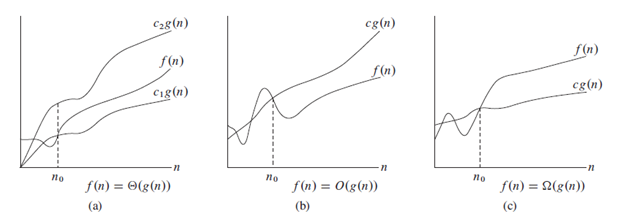
\includegraphics[width=.7\linewidth]{figures/big_o}
	\caption{Wizualizacja asymptotycznego ograniczenia funkcji. Źródło: Cormen et al.}
\end{figure}

\subsection{Standardowe rzędy wielkości funkcji}

\begin{table}[]
\caption{Popularne rzędy wielkości wraz z nazewnictwem}
\centering
\begin{tabular}{@{}ll@{}}
\toprule
Klasa & Opis \\ \midrule
$\Theta(0)=0$ & brak potrzebnych operacji \\
$\Theta(1)$ & stała \\
$\Theta(\log n)$ & logarytmiczny \\
$\Theta((\log n)^c)$ & polilogarytmiczny \\
$\Theta(n)$ & liniowy \\
$\Theta(n \log n)$ & log-liniowy (quasi-liniowy) \\
$\Theta(n^2)$ & kwadratowy \\
$\Theta(n^c)$ & wielomianowy \\
$\Theta(c^n)$ & wykładniczy \\
$\Theta(n!)$ & silnia \\ 
$\Theta(n^n)$ & ... \\ \bottomrule
\end{tabular}
\end{table}


\begin{table}[]
\caption{Czas potrzebny na wykonanie funkcji o różnej złożoności. Źródło: DZone}
\centering
\begin{tabular}{@{}rrrrrrrr@{}}
\toprule
$n$ & $O(1)$ & $O(\log n)$ & $O(n)$ & $O(n \log n)$ & $O(n^2)$ & $ n^2 +100n$ & $O(n3)$ \\ \midrule
1 & 1 & 1 & 1 & 1 & 1 & 101 & 1 \\
2 & 1 & 1 & 2 & 2 & 4 & 204 & 8 \\
4 & 1 & 2 & 4 & 8 & 16 & 416 & 64 \\
8 & 1 & 3 & 8 & 24 & 64 & 864 & 512 \\
16 & 1 & 4 & 16 & 64 & 256 & 1,856 & 4,096 \\
1,024 & 1 & 10 & 1,024 & 10,240 & 1,048,576 & 1,150,976 & 1,073,741,824 \\
\bottomrule
\end{tabular}
\end{table}

\begin{figure}
	\centering
	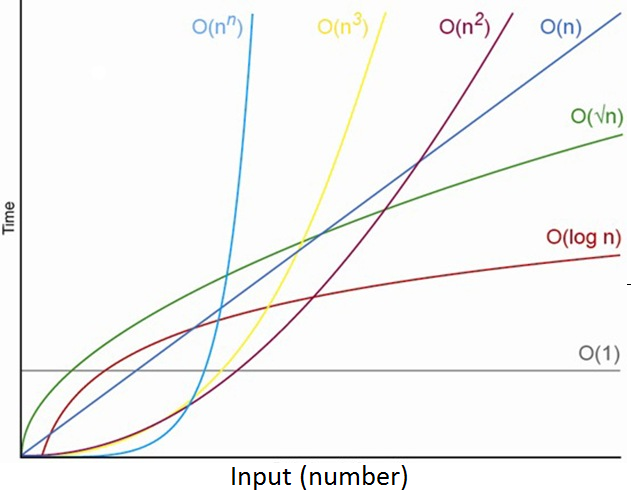
\includegraphics[width=.4\textwidth]{figures/complexities}
	\caption{Wizualizacja różnych klas złożoności funkcji. Źródło: Stack Overflow}
\end{figure}

\section{Struktury danych}
\subsection{Kolejka}

\subsection{Stos}

\subsection{Drzewa}
Drzewo to graf skierowany spójny i acykliczny.

\subsection{Drzewa BST}
Klasa drzewa i elementu drzewa:
\begin{minted}{python}
class Tree():                         # drzewo
  def __init__(self, root=None):      # konstruktor drzewa, w pythonie dla klas pierwszy argument jest pomijany (to zawsze self), a jedynym "prawdziwym" argumentem jest korzeń (domyślnie pusty)
    self.root = root                  

class Node:                           # węzeł drzewa
  def __init__(self, k, left, right, parent=None): # konstruktur (klucz, lewe dziecko, prawe dziecko, rodzic (domyślnie pusty))
    self.parent = parent              # rodzic 
    self.key = k                      # wartość przechowywana w tym węźle
    self.left = left                  # wskaźnik na lewe poddrzewo
    self.right = right                # wskaźnik na prawe poddrewo
  def __str__(self):                  # metoda zamieniająca drzewo na łańcuch znaków (przydatna przy printowaniu)
    return "Jestem węzłem drzewa i przechowuję wartość {}".format(self.key)
\end{minted}
Tworzenie drzewa:
\begin{minted}{python}
tree = Tree(root=Node(6, 
                      Node(5, 
                          Node(2, None, None), 
                          Node(5, None, None)), 
                      Node(7, 
                          None, 
                          Node(8, None, None))
            ))
\end{minted}
Przechodzenie drzewa inorder:
\begin{minted}{python}
def inorderTreeWalk(x, indent=1):
  if x is not None:
    inorderTreeWalk(x.left, indent + 1)
    print(('  ' * indent) + str(x.key))
    inorderTreeWalk(x.right, indent + 1)
    
inorderTreeWalk(tree.root)  # korzeń najbardziej wysunięty na lewo
\end{minted}
Szukanie elementu po wartości:
\begin{minted}{python}
def treeSearch(x, k):
  if x is None or k == x.key:
    return x
  if k < x.key:
    return treeSearch(x.left, k)
  else:
    return treeSearch(x.right, k)
    
nodeWithSeven = treeSearch(tree.root, 7)
print(nodeWithSeven)
\end{minted}

\begin{minted}{python}
	
\end{minted}

\begin{minted}{python}
	
\end{minted}

\subsection{Kodowanie Huffmana}


\section{Algorytmy sortowania}

\subsection{Sortowanie bąbelkowe}

\subsection{Heapsort -- sortowanie przez kopcowanie}

\begin{algorithm}
    \caption{Sortowanie szybkie (przykład z książki -- liczymy od 1!)}
    \label{alg:quicksort}
    \begin{algorithmic}[1] % The number tells where the line numbering should start
        \Function{Parent}{$i$} 
            \State \Return $\lfloor i/2 \rfloor$
        \EndFunction
        	\Function{Left}{$i$} 
            	\State \Return $2i$
        \EndFunction
        	\Function{Right}{$i$} 
            	\State \Return $2i+1$
        \EndFunction
    \end{algorithmic}
\end{algorithm}

W kopcach typu \emph{max} mamy dla każdego $i$, które nie jest korzeniem $A[\Call{Parent}{i} \geq A[i]$. Kopiec mający $n$ elementów ma wysokość $\Theta (\log_2 n)$


\section{Wstęp do teorii grafów i związane z nią algorytmy}
\subsection{Grafy oraz przechodzenie przez nie}
\subsection{Algorytm Dijkstry}
\subsection{Algorytm Prima}

\section{Wyszukiwanie wzorca w tekście}

\subsection{Wyszukiwanie naiwne}

\subsection{Algorytm Aho-Corasik}

\section{NP-zupełność. Czy P=NP?}
\end{document}